\section{Consistency Failure Analysis}
\label{sec:failures}

\begin{table}[t]
\centering
\caption{\textbf{Frozen.} Qwen violation multiplicity (H4). BCR~$=$~0 reflects multi-constraint failure.}
\label{tab:violations}
\small
\begin{tabular}{lrrr}
\toprule
System & Mean viol./bundle & Frac.\ exactly one & Frac.\ multiple \\
\midrule
B1 / B3 & 3.59 & 0.031 & 0.969 \\
B4 BM25 & 3.33 & 0.177 & 0.823 \\
H0 reference & 3.50 & 0.000 & 1.000 \\
\bottomrule
\end{tabular}
\end{table}

\begin{figure}[t]
\centering
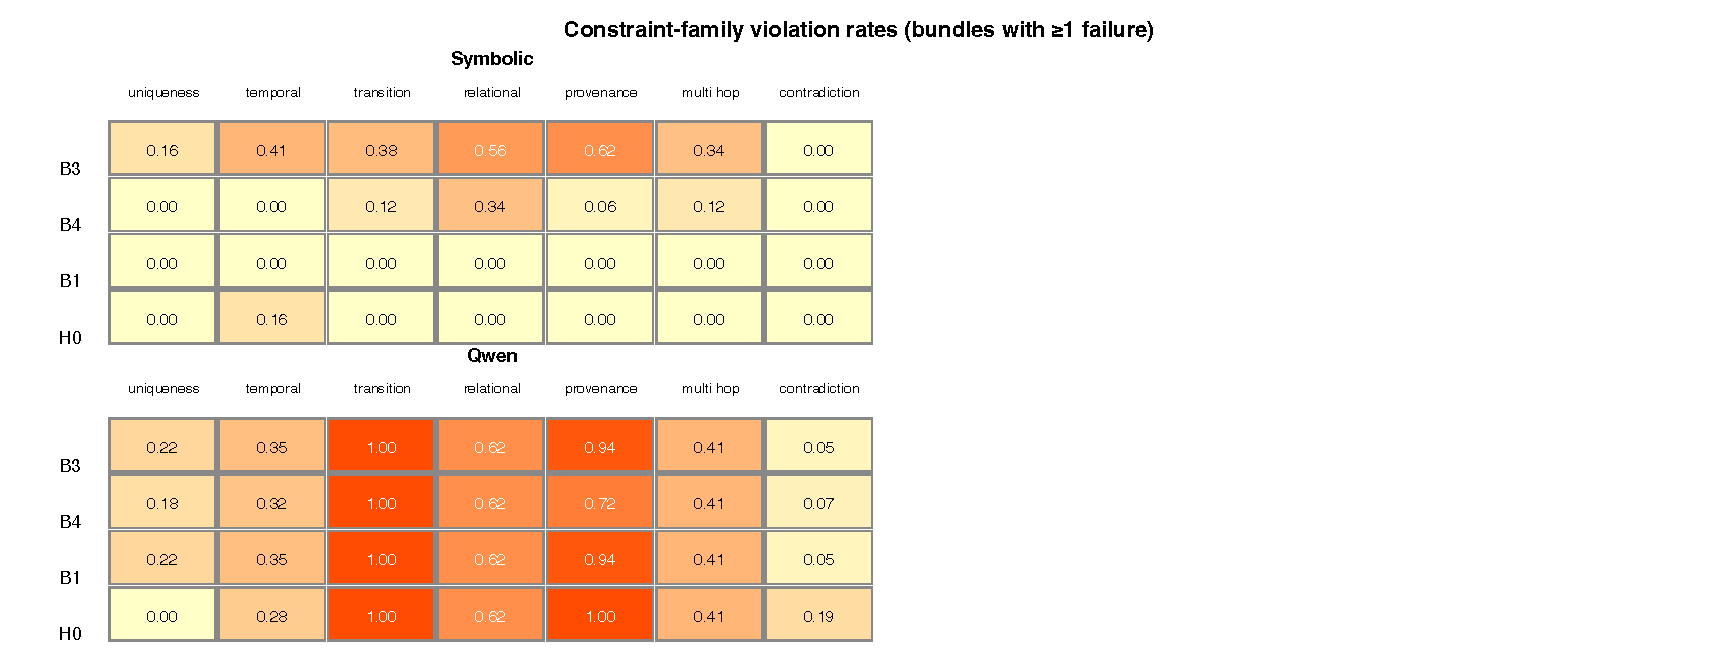
\includegraphics[width=0.92\linewidth]{figures/fig4-constraint-family-heatmap.pdf}
\caption{Constraint-family violation rates (frozen). Takeaway: Qwen failures concentrate on transition/provenance.}
\label{fig:constraints}
\end{figure}

Abstention is high for B1/B3 (0.728), lower for B4 (0.579) and H0 (0.483). Extended tables: Appendix~\ref{app:extrafigs}.
